
\chapter{Multidimensional Nonuniform Gap Sampling}

\begin{quote}
{\it
  Anyone who considers arithmetical methods of producing random digits is,
  of course, in a state of sin.}
\\\\
 -- John von Neumann
\end{quote}

\section{Introduction}

\begin{doublespace}
The use of nonuniform sampling in multidimensional NMR is rapidly becoming
standard practice in most biomolecular solution-state experiments, thanks in
large part to recent developments in fast reconstruction algorithms, novel
sampling schemes, and the continually declining cost of computing power
\cite{mobli:pnmrs2014}. The potential benefits of collecting a subset of the
full Nyquist grid -- including increased sensitivity and signal-to-noise,
improved resolution, and reduced experiment time -- have received significant
attention \cite{
  rovnyak:jmr2004, rovnyak:jbnmr2004, kazimierczuk:angew2011,
  hyberts:jbnmr2013, palmer:jbnmr2014} in recent years as a consequence.
\\\\
One intriguing result of recent investigations into the parameters of NUS
experiments is the use of random deviates for generating sampling schedules
\cite{hoch:jmr2008}. In fully random sampling schemes, a subset of Nyquist
grid points is drawn from a probability density function that varies over the
grid, producing a sampling schedule with a desired distribution of points.
Common fully random sampling schemes utilize uniform, exponential, Gaussian
and envelope-matched probability densities
\cite{palmer:jbnmr2014,schuyler:jbnmr2011}. While randomization is a simple
means of reducing the artifacts due to aliasing of nonuniformly spaced samples,
it turns the already complex task of schedule generation into that of selecting
a schedule from an ensemble of possibilities, each of which performs
differently in practice \cite{hyberts:jacs2010,mobli:jmr2015}. Several ad hoc
metrics have been proposed to assess the relative performance sampling
schedules, but no universally accepted metric exists to guide the selection
of a stochastic schedule from its ensemble \cite{mobli:jmr2015,aoto:jmr2014}.
Without a priori knowledge of the frequency and decay rate distributions of
the signals to be measured, it is difficult to reliably quantify sampling
schedule performance \cite{mobli:pnmrs2014,schuyler:jbnmr2011}. As a result,
numerous recent attempts have been made to reduce or remove pseudorandom
seed-dependent variability from nonuniform sampling algorithms
\cite{kazimierczuk:jmr2007,hyberts:jacs2010,eddy:jmr2012,mobli:jmr2015}.
Such efforts are an important step towards increasing the practical utility
of nonuniform sampling in everyday spectroscopic experiments.
\\\\
Through an empirical analysis of Forward Maximum Entropy (FM) reconstructions
of randomly sampled data, Hyberts et al. proposed the use of constrained
Poisson random deviates to define the \emph{gaps} between sampled points
in a Nyquist grid \cite{hyberts:jacs2010}. The FM reconstruction residuals
of these so-named Poisson-gap schedules exhibited a markedly lower dependence
on seed value than unconstrained random sampling methods. While Poisson-gap
sampling yields high-quality reconstructions of NUS spectral data, its average
behavior is not well-understood, its implementation for multidimensional
Nyquist grids is unclear
\cite{hyberts:tcc2012,hyberts:jbnmr2012,hyberts:jmr2014},
and its relationship -- if any -- to fully random sampling is unknown.
To meet this need, this work describes in detail the deterministic generation
of sinusoidally weighted multidimensional gap schedules that model the average
behavior of stochastic Poisson-gap (PG) sampling. An expectation sampling
probability distribution is also derived that reflects the average weighting
obtained using one-dimensional Poisson-gap sampling schedules.
\\\\
Among the myriad of different sampling schemes proposed for NUS data
collection \cite{maciejewski:tcc2012}, burst-mode sampling similarly concerns
itself with gaps between sampled grid points. Unlike Poisson-gap sampling,
which aims to minimize the \emph{length} of gaps, burst-mode sampling aims
to minimize the \emph{number} of gaps while keeping the effective dwell time
low \cite{maciejewski:jmr2009}. We leverage the complementarity of burst-mode
and Poisson-gap sampling in our deterministic gap sampling algorithm to
describe a novel sampling scheme that simultaneously seeks to bias sample
collection to early times, minimize the number of long gaps between densely
sampled regions, and minimize the largest gap length in the schedule. The
resulting method, called sine-burst (SB) sampling, exhibits the high
performance of Poisson-gap sampling while retaining the bijective mapping
between inputs and outputs offered by deterministic methods.
\end{doublespace}

\section{Theory}

\subsection{Poisson-gap Sequences}

\begin{doublespace}
Gap schedules on a one-dimensional Nyquist grid are effectively finite integer
sequences, computed from the following recurrence relation:
\begin{equation}
x_{i+1} = x_i + \lfloor g(x_i) \rfloor + 1
\end{equation}
where $x_i$ is the grid index of the $i$-th term in the sequence and $g(x_i)$
is the ``gap equation'' that defines the distance between terms. The first term
in the sequence, $x_1$, is set to 1 and subsequent terms are computed until
their value exceeds $N$, the size of the grid. The gap equation $g(x)$ may be
any non-negative function, and may be loosely interpreted as inversely related
to the local sampling density at the grid index $x_i$. Thus, when the gap
equation equals zero for all grid indices, gap sampling will yield a uniformly
sampled grid.
\\\\
Poisson-gap sequences treat the gap equation as a Poisson random deviate
having a rate parameter that varies as either a quarter- or half-sinusoid
over the grid indices:
\begin{equation}
g_{PG}(x_i) \sim \mathrm{Pois} \left\{
 \Lambda \sin \left(
  \frac{\pi}{2} \theta_i
 \right)
\right\}
\end{equation}
where $\Lambda$ is a scaling factor that determines the global sampling
density and $\theta_i$ is the fractional grid index that varies from 0 to 1
over the grid extents:
\begin{equation}
\theta_i = \frac{x_i}{N}
\end{equation}

In all following descriptions of Poisson-gap methods, we shall restrict our
attention to rate parameters which vary as quarter-sinusoids, where the
fractional grid index is multiplied by a factor of one-half $\pi$. This choice
of sinusoidal weight produces schedules that are heavily biased to earlier
grid points. Using a factor of $\pi$ produces half-sinusoidal rate parameters
and schedules that are more densely sampled at both early and late grid points.
\\\\
Because the expected value of a Poisson distribution is equal to its rate
parameter, one may trivially construct a deterministic sinusoidally weighted
gap sampler (sine-gap; SG) by setting the gap equation equal to the scaled
quarter-sinusoid from equation 2.2, as follows:
\begin{equation}
g_{SG} = \Lambda \sin \left( \frac{\pi}{2} \theta_i \right)
\end{equation}

By construction, gap sampling schedules computed according to $g_{SG}$ will
describe the average behavior of $g_{PG}$. This is readily verified in one
dimension by generating a sufficiently large set of stochastic Poisson-gap
schedules and comparing the mean value of each sequence term to that of a
sine-gap schedule (\figref{2.1}{Figure 2.1}). Sine-gap schedules
lie centrally within the Poisson-gap ensemble, while other schedules
unrelated to Poisson-gap deviate substantially from the confidence
region of the ensemble.
\end{doublespace}

\begin{figure}[ht!]
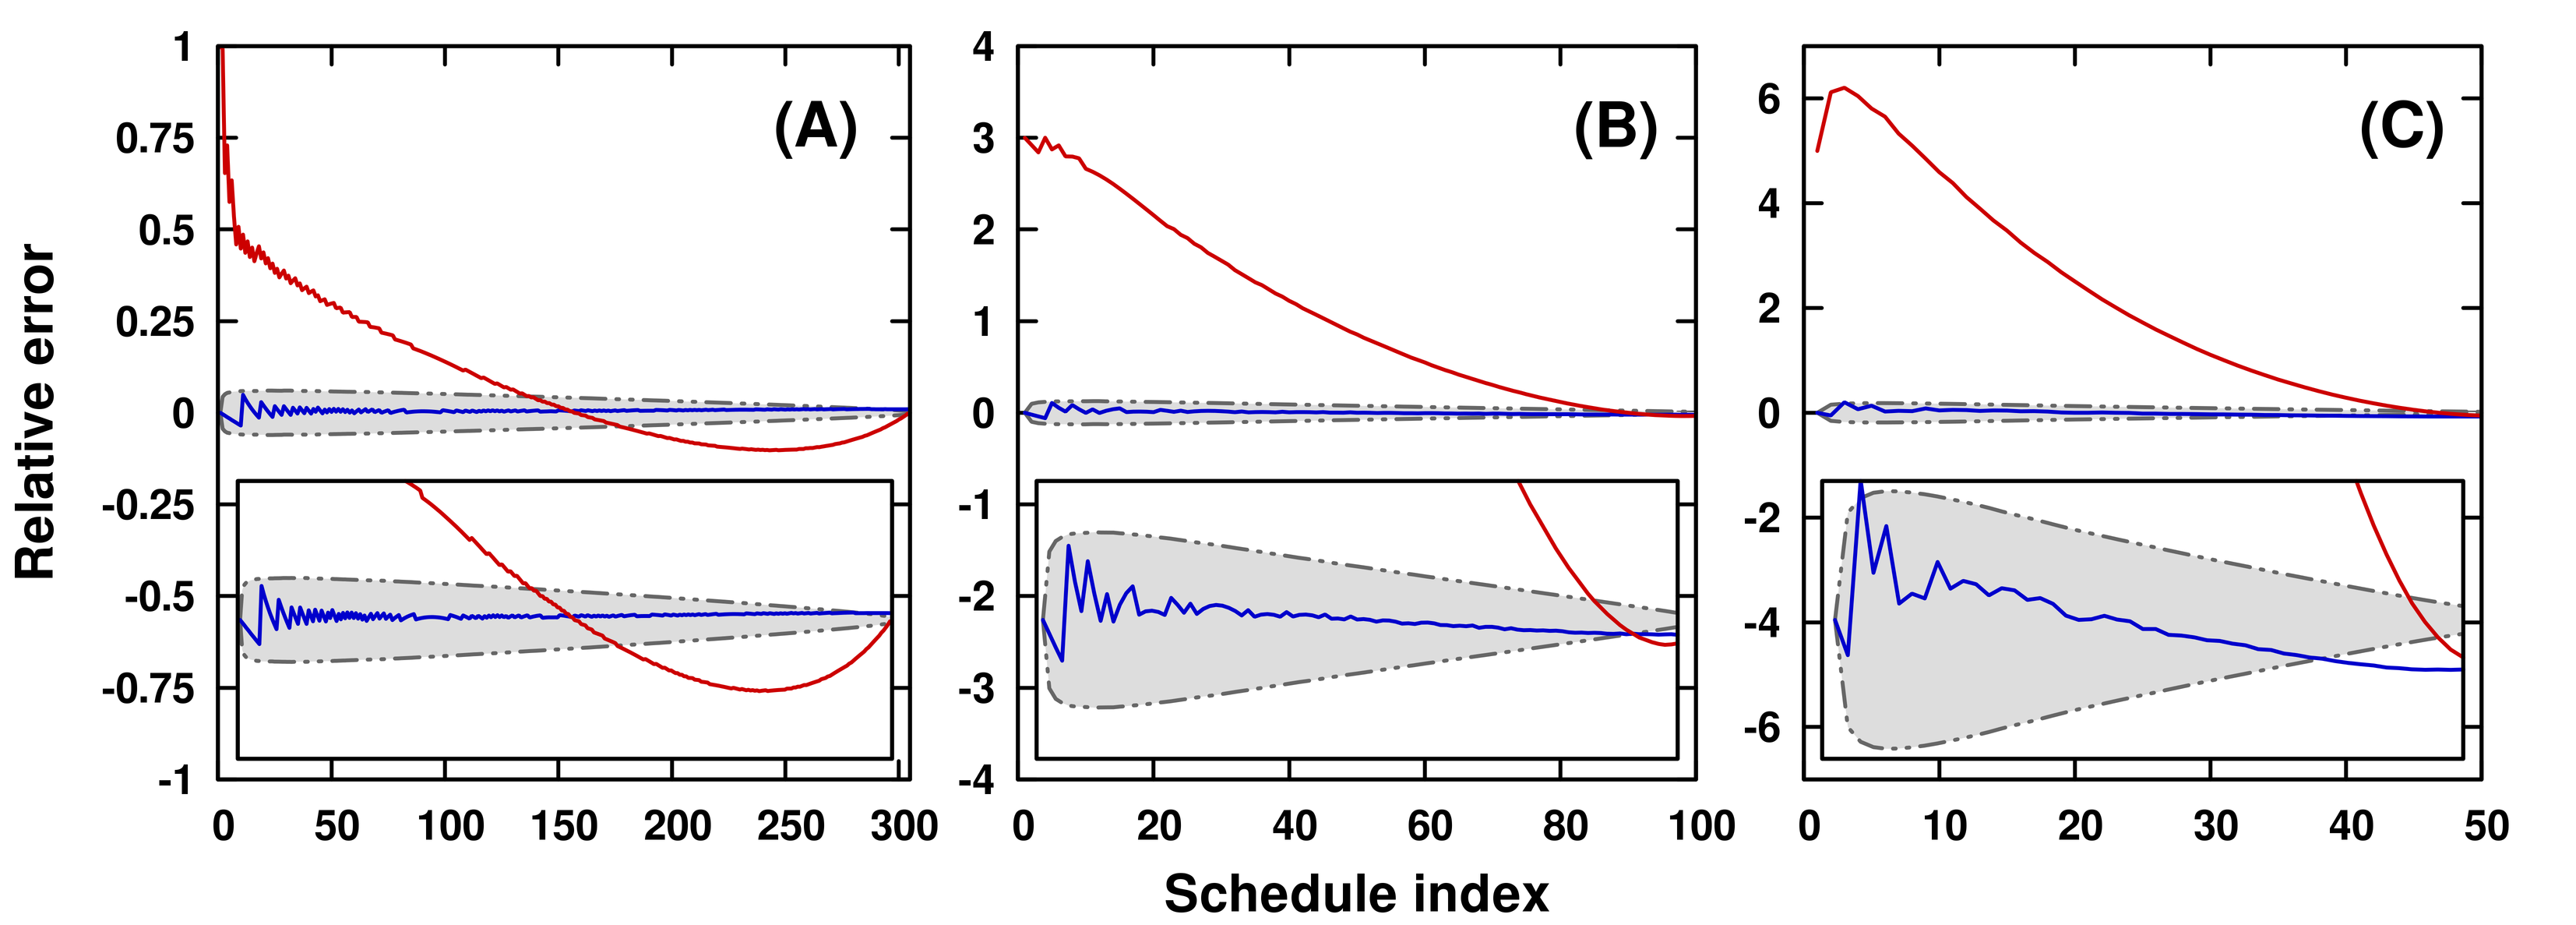
\includegraphics[width=6in]{figs/dgs/01-avepg.png}
\caption
      [Agreement between Poisson-gap and sine-gap Sequences.]{
  {\bf Agreement between Poisson-gap and sine-gap Sequences.}
  \\
  Relative errors between sine-gap (blue lines) and deterministic exponential
  (red lines) schedules with respect to the average Poisson-gap schedule at
  ({\bf A}) 30\% density, ({\bf B}) 10\% density and ({\bf C}) 5\% density.
  Confidence intervals indicating plus or minus one standard deviation of the
  Poisson-gap ensemble are shown as grey shaded regions. The vertical axes of
  all inset plots range from $-0.2$ to $0.2$. Because the sine-gap schedules
  describe the average behavior of the Poisson-gap equation, they lie
  centrally within the Poisson-gap ensemble, while any other schedule
  unrelated to Poisson-gap (e.g. exponential) does not.
}
\label{figure.2.1}
\end{figure}

\subsection{Multidimensional Gap Sampling}

\begin{doublespace}
Gap schedules on a Nyquist grid having at least two dimensions are generated
by placing multiple one-dimensional sub-schedules onto the grid, each with a
different direction and offset from the grid origin. In practice, this process
is accomplished recursively, with planes built up from vectors, cubes built up
from planes, and so forth. Initially, recursion begins on the entire grid. At
each level of recursion, sub-grids are constructed by ``masking off'' each
available grid direction in turn and constructing the remaining unmasked
directions. For example, a three-dimensional $xyz$ cube will be constructed
from repeated sequences of $yz$, $xz$ and $xy$ planes, and each $xy$ plane
will be constructed from repeated sequences of $y$ and $x$ vectors. Once a
round of sub-grid construction has been performed along each direction, the
sub-grid offset is incremented and the process is repeated until no more
sub-grids remain at the current level of recursion. The following executable
pseudocode provides a more precise definition of the recursive gap sampling
algorithm:
\end{doublespace}

\begin{algorithm}[H]
\caption{Multidimensional Gap Sampling Algorithm}
\label{algorithm.2.1}
\begin{python}
def build(N, origin, mask):
  D = len(N)
  if sum(mask) == 1:
    direction = mask.index(1)
    dirstring = ['x', 'y', 'z'][direction]
    print('sequence along ' + dirstring + ' at origin ' + origin)
    return

  suborigin = [0,] * D
  submask = [0,] * D
  done = False
  offset = 0

  while not done:
    done = True
    for direction in range(D):
      if mask[direction] != 1 or offset >= N[direction]:
        continue

      done = False
      for d in range(D):
        if d != direction and mask[d] == 1:
          submask[d] = 1
        else:
          submask[d] = 0

        if d == direction:
          suborigin[d] = offset
        else:
          suborigin[d] = origin[d]

      build(N, suborigin, submask)
    offset = offset + 1

build([8, 4, 4], [0, 0, 0], [1, 1, 1])
\end{python}
\end{algorithm}

\begin{doublespace}
Creation of multidimensional gap schedules requires a slight modification to
the fractional index, which now assumes the following form:
\begin{equation}
\theta_i = \frac{x_i + \sum_{d=1}^D O_d}{\sum_{d=1}^D N_d}
\end{equation}
where $O_d$ and $N_d$ are the origin and grid size along direction $d$,
respectively. The above equation is referred to as ``ADD'' mode in the context
of stochastic Poisson-gap sampling, and effectively results in multidimensional
schedules that exhibit triangular forms \cite{hyberts:jmr2014}. It is worthy of
mention that, in the one-dimensional case, equation 2.5 reduces to equation
2.3.
\\\\
Finally, whether the Nyquist grid is one- or many-dimensional, a value of the
global scaling factor $\Lambda$ must be determined that yields the desired
number of sampled grid points. Our gap sampling implementation, like the
existing Poisson-gap method, iteratively rebuilds new schedules until
$\Lambda$ has been suitably optimized.
\end{doublespace}

\subsection{Burst Augmentation}

\begin{doublespace}
Recent statistical descriptions of the discrete Fourier transform have shown
that the bandwidth of a nonuniformly sampled signal is related to the greatest
common factor of the gaps between sampled grid points
\cite{bretthorst:cmr2008}. One proposed method of increasing bandwidth and
reducing artifacts in NUS data is to sample in multiple short bursts having
zero gap length \cite{maciejewski:jmr2009}. Using gap sampling, this may be
accomplished by modulating the gap equation between zero and its maximum value
several times over the Nyquist grid, like so:
\begin{equation}
g_{SB}(x_i; d) = \Lambda
 \sin \left( \frac{\pi}{2} \theta_i \right)
 \sin^2 \left( \frac{\pi}{4} N_d \theta_i \right)
\end{equation}

The sine-burst gap equation $g_{SB}$ combines the sinusoidal forward-biasing
and minimized gap lengths of Poisson-gap sampling with the minimized effective
dwell time of burst-mode sampling, and does not require the use of random
deviates to achieve reasonable artifact suppression.
\end{doublespace}

\begin{figure}[ht!]
\begin{center}
  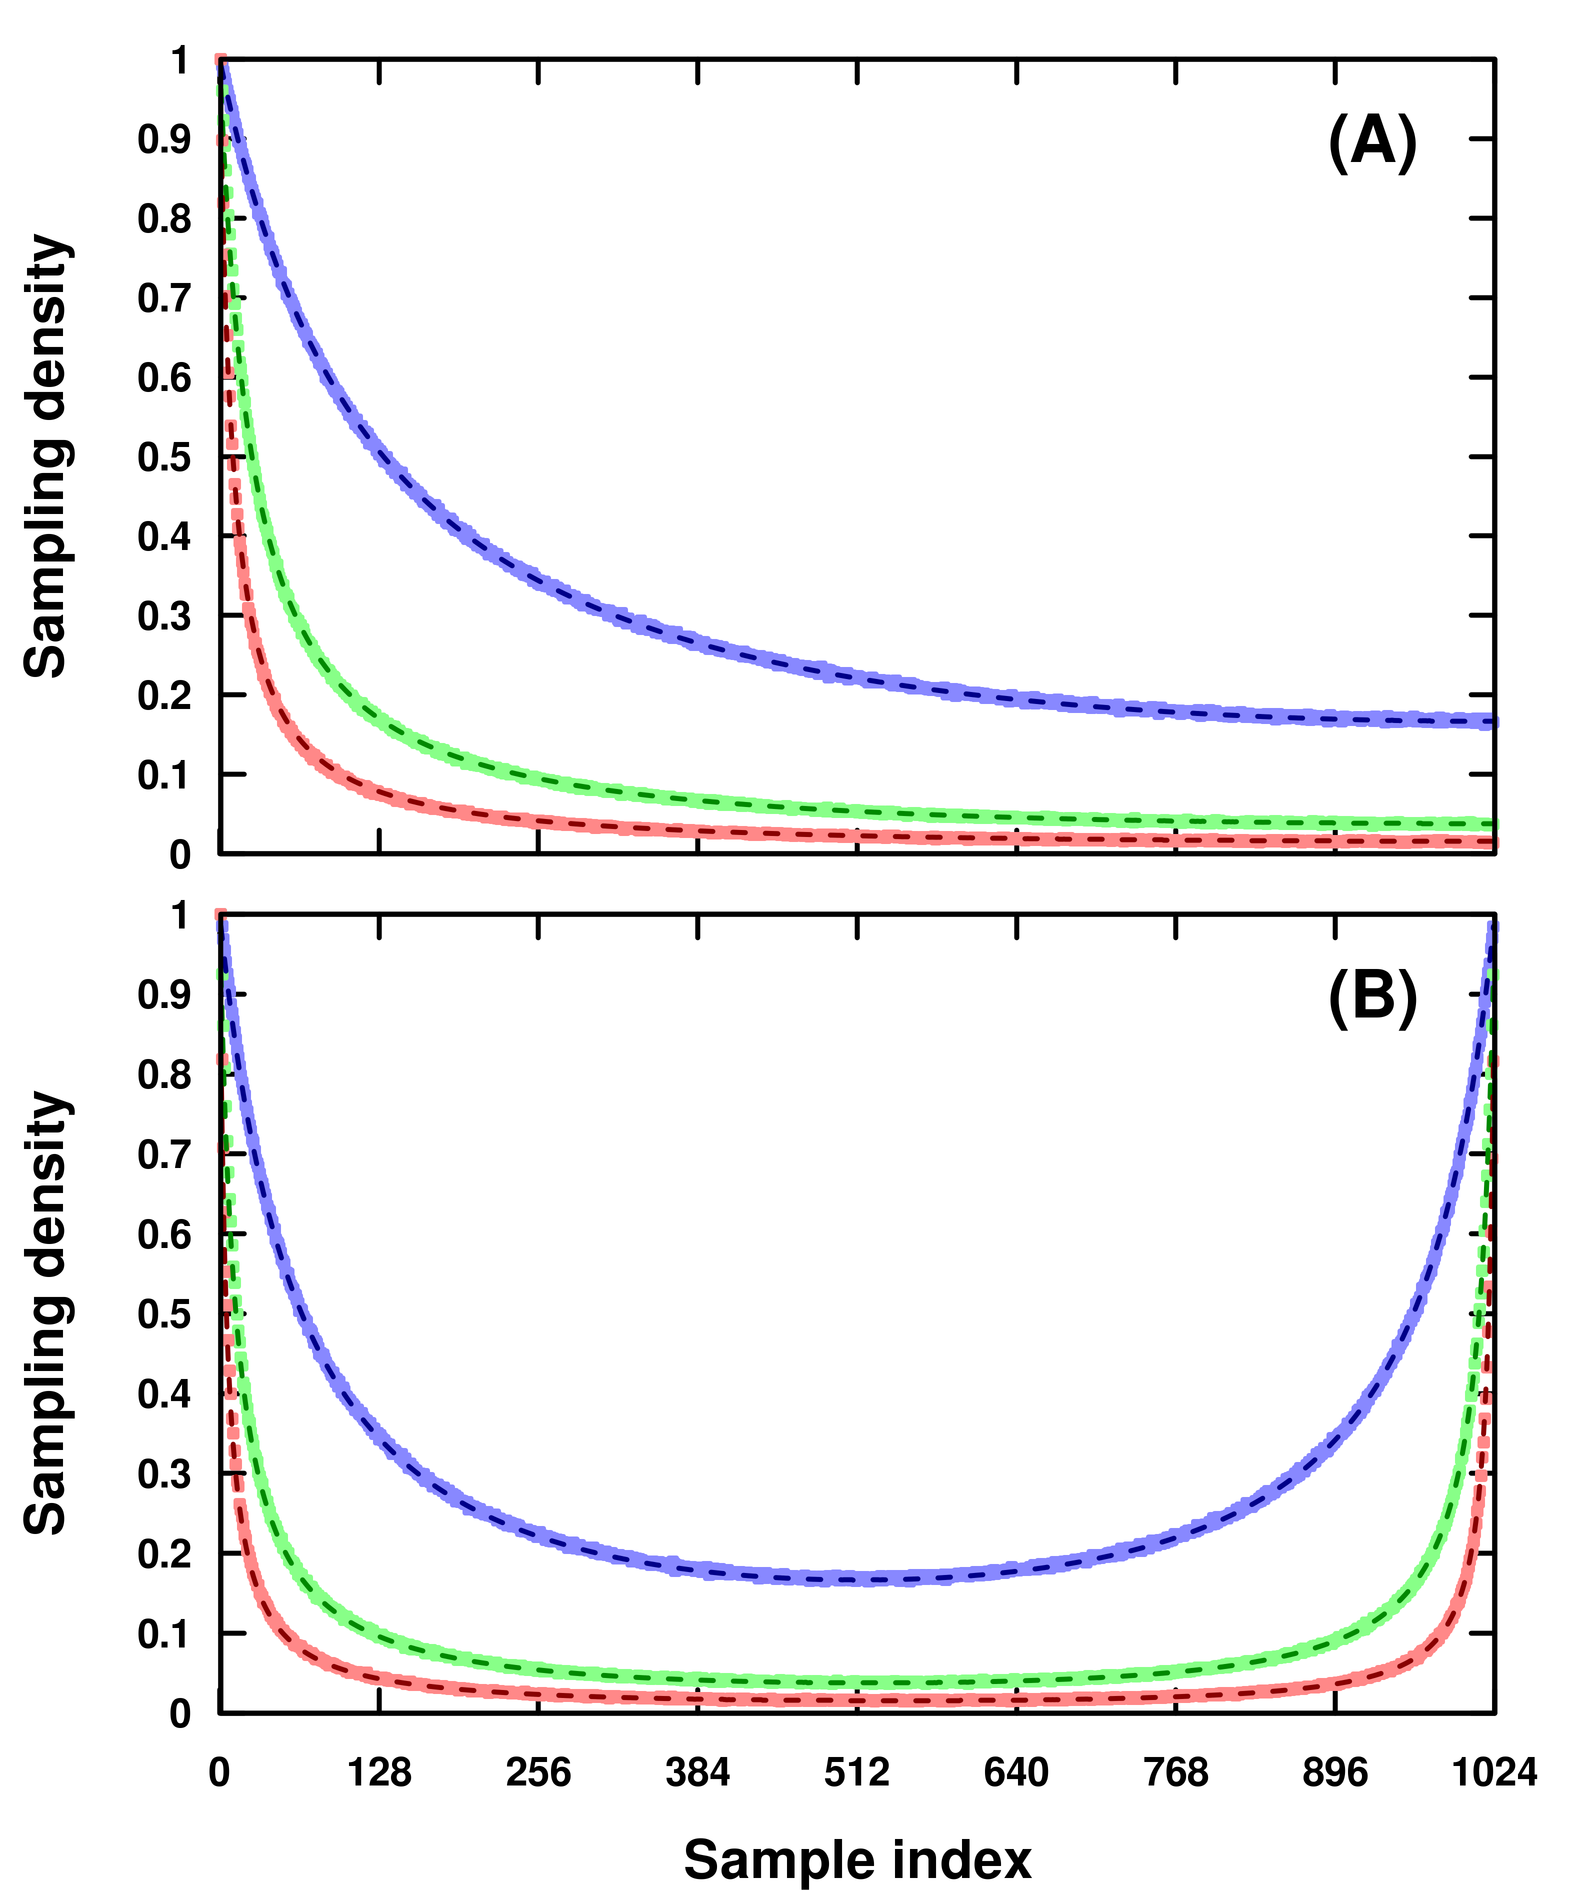
\includegraphics[width=4.5in]{figs/dgs/02-expect-1d.png}
\end{center}
\caption
      [Poisson-gap 1D Expectation Sampling Distributions.]{
  {\bf Poisson-gap 1D Expectation Sampling Distributions.}
  \\
  Expectation sampling distributions computed by averaging 50,000
  one-dimensional Poisson-gap schedules of varying densities, with
  quarter-sinusoidal ({\bf A}) and half-sinusoidal ({\bf B}) weightings.
  The lighter blue, green and red points were computed from schedules having
  30\%, 10\% and 5\% sampling density, respectively. The dashed lines overlaid
  on each set of points correspond to the analytic sampling distribution
  (equation 2.11) derived from $g_{PG}$. Values of $\Lambda$ were 5.0, 25.4
  and 62.9 for 30\%, 10\% and 5\% sampling density, respectively.
}
\label{figure.2.2}
\end{figure}

\subsection{Expectation Sampling Distributions}

\begin{doublespace}
One disadvantage of stochastic gap equations is that they provide no direct
measure of how likely each Nyquist grid point is to be sampled. While one may
speculate on the approximate weighting obtained by a given gap equation,
quantitation of the expectation of the sampling distribution requires the
construction and averaging of a large number of sampling schedules
(cf. \figref{2.2}{Figures 2.2}, \figref{2.3}{2.3} and \figref{2.4}{2.4}).
Fortunately, the expectation sampling distribution of a given gap equation
may be analytically obtained by computing the probability of sampling each
point on the grid using a recursive formula. We define an expectation
sampling distribution $p(i)$ that varies over a one-dimensional Nyquist
grid of $N$ points as follows:
\begin{equation}
p(i) = \sum_{k=1}^{i-1} p(i \mid i-k) p(i-k)
\end{equation}
where $p(i \mid i-k)$ is the probability of grid point $i$ being emitted from
grid point $i-k$, which requires a gap size of $k-1$:
\begin{equation}
p(i \mid i-k) = \mathrm{Pr}\left\{
 \lfloor g(i-k) \rfloor = k - 1
\right\}
\end{equation}

In other words, the probability of sampling any given grid point is the
weighted sum of the probabilities of arriving at that point from all prior
points. In the case of Poisson-gap sampling, the gap equation is a Poisson
random deviate:
\begin{equation}
\mathrm{Pr}\left\{ \lfloor g(x_i) \rfloor = k - 1 \right\} =
 \frac{\lambda(x_i)^{k-1}}{(k-1)!} e^{-\lambda(x_i)}
\end{equation}
where the rate parameter $\lambda(x_i)$ varies sinusoidally over the Nyquist
grid:
\begin{equation}
\lambda(m) = \Lambda \sin \left( \frac{\pi m}{2 N} \right)
\end{equation}

By combining the above four equations, we arrive at the sampling distribution
of a one-dimensional Poisson-gap sequence:
\begin{equation}
p(i) = \sum_{k=1}^{i-1} \frac{\Lambda^{k-1}}{(k-1)!}
 \sin^{k-1} \left( \frac{\pi [i-k]}{2 N} \right)
 \exp\left\{
  -\Lambda \sin \left( \frac{\pi [i-k]}{2 N} \right)
 \right\}
p(i-k)
\end{equation}

As in the case of gap sampling, the sampling distribution produced by equation
2.11 is parameterized only by the scaling factor $\Lambda$, where larger values
yield more forward-biased schedules (\figref{2.2}{Figure 2.2}). We refer
to this equation as the ``expectation'' Poisson-gap sampling distribution
because it describes the expected value of the probability of sampling any
Nyquist grid point, and is not itself useful for generating schedules that
obey $g_{PG}$.
\end{doublespace}

\begin{figure}[ht!]
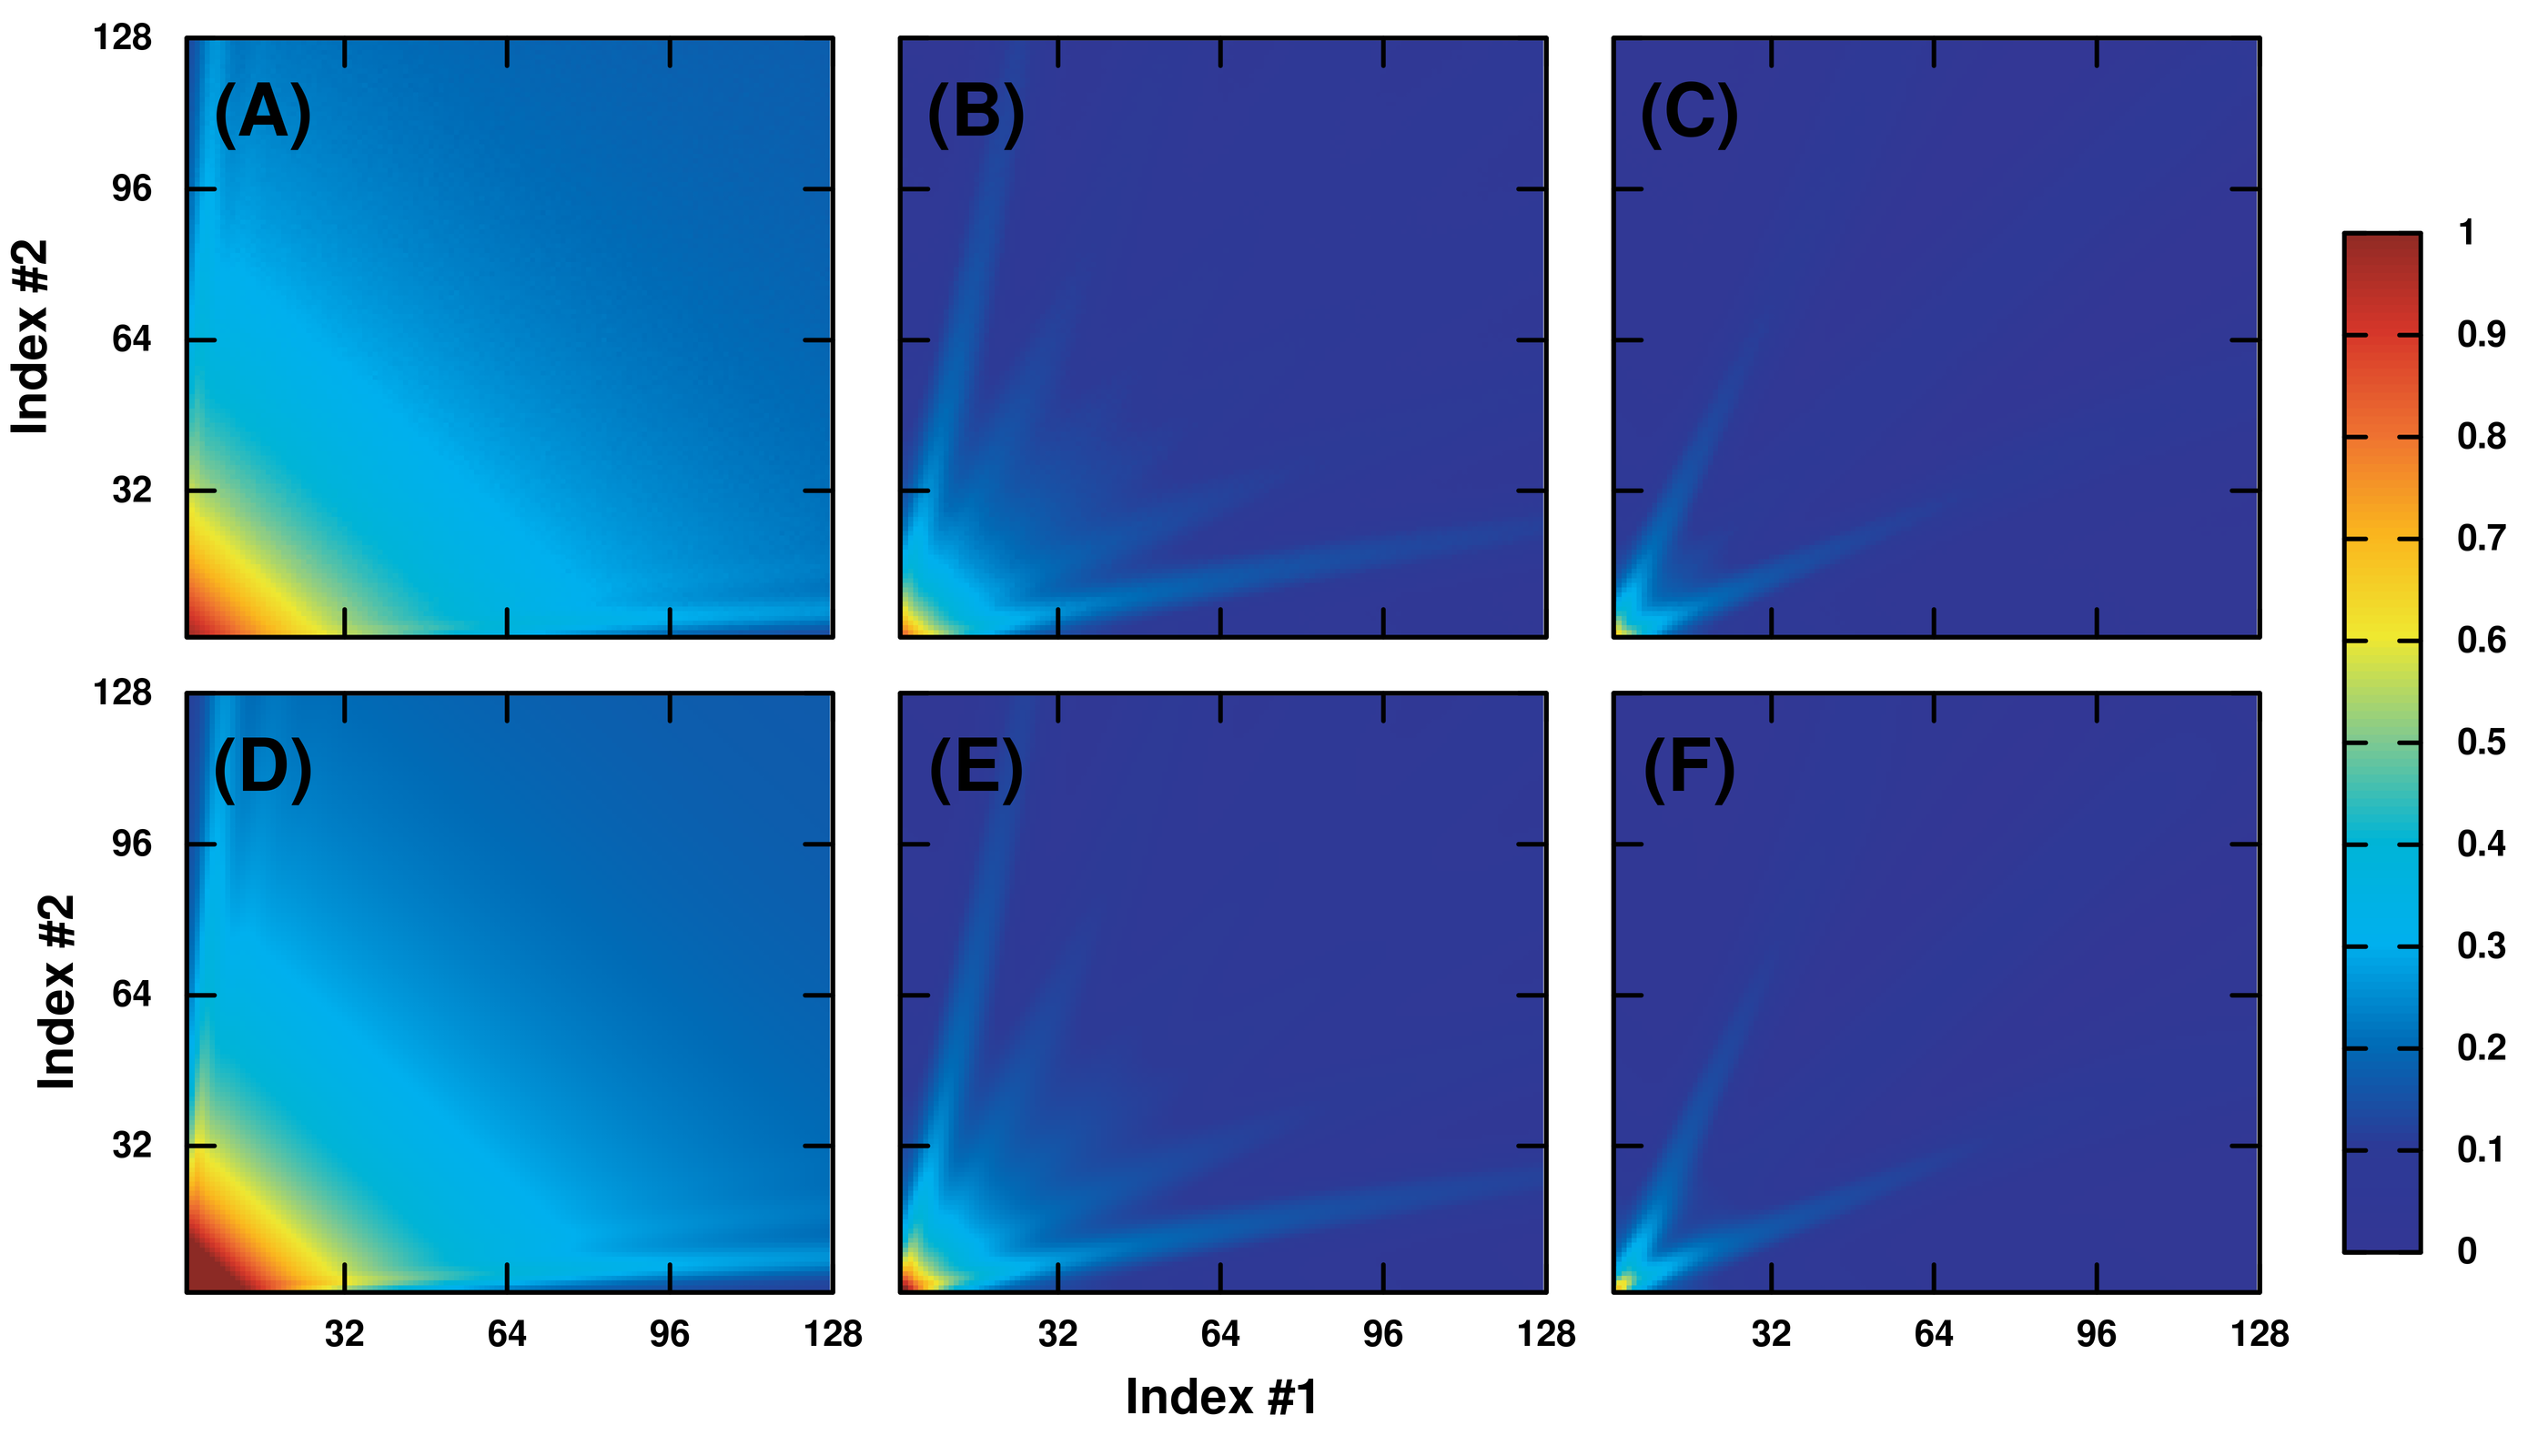
\includegraphics[width=6in]{figs/dgs/03-expect-2d.png}
\caption
      [Poisson-gap 2D Expectation Sampling Distributions.]{
  {\bf Poisson-gap 2D Expectation Sampling Distributions.}
  \\
  Expectation sampling distributions of two-dimensional Poisson-gap schedules
  computed in strict accordance to Algorithm 2.1. Top panels were produced by
  averaging 50,000 two-dimensional schedules, and bottom panels were computed
  using equation 2.12 with appropriate substitutions of the Poisson
  probability mass function. Sampling densities of 30\%, 10\% and 5\% are
  shown in panels ({\bf A}, {\bf D}), ({\bf B}, {\bf E}) and
  ({\bf C}, {\bf F}), respectively.
}
\label{figure.2.3}
\end{figure}

\begin{figure}[ht!]
\includegraphics[width=6in]{figs/dgs/04-expect-hyb.png}
\caption
      [Poisson-gap 2D Expectation Sampling Distributions.]{
  {\bf Poisson-gap 2D Expectation Sampling Distributions.}
  \\
  Expectation sampling distributions computed by averaging 50,000
  two-dimensional Poisson-gap schedules generated using code provided by
  Hyberts and Wagner. Sampling densities of 30\%, 10\% and 5\% are
  shown in panels ({\bf A}), ({\bf B}) and ({\bf C}), respectively.
}
\label{figure.2.4}
\end{figure}

\subsection{Multidimensional Expectation Sampling Distributions}

\begin{doublespace}
Extension of equation 2.11 to compute the expectation sampling distributions
of stochastic gap equations in two or more dimensions follows from the fact
that sampling along each direction is essentially independent of other
directions within the presented gap sampling framework. As a consequence,
the probability of sampling any multidimensional grid point is therefore the
sum of sampling that point along each grid direction. For a two-dimensional
grid $(i_1,i_2)$, the expectation sampling distribution is the sum of the
probability matrices $p_1(i_1,i_2)$ and $p_2(i_1,i_2)$:
\begin{align}
p_1(i_1,i_2) =& \sum_{k=1}^{i_1-1} p(i_1,i_2 \mid i_1-k,i_2) p_1(i_1-k,i_2)
 \nonumber \\
p_2(i_1,i_2) =& \sum_{k=1}^{i_2-1} p(i_1,i_2 \mid i_1,i_2-k) p_2(i_1,i_2-k)
 \nonumber \\
p(i_1,i_2) =&\: p_1(i_1,i_2) + p_2(i_1,i_2)
\end{align}

\figref{2.3}{Figure 2.3} illustrates the expectation Poisson-gap sampling
distribution on two-dimensional Nyquist grids. It is important to note that
the Poisson-gap sampler originally proposed by Hyberts et al. does not
strictly follow Algorithm 2.1, because its sampling of each dimension is
dependent upon which points in other dimensions have been previously sampled.
This divergence between multidimensional Poisson-gap and Poisson-gap
constructed using Algorithm 2.1 is observed by comparison of
\figref{2.3}{Figures 2.3} and \figref{2.4}{2.4}, and is only
truly apparent at very low sampling densities.
\end{doublespace}

\begin{figure}[ht!]
\includegraphics[width=6in]{figs/dgs/05-psf.png}
\caption
      [Comparison of Gap Sampling Schedules.]{
  {\bf Comparison of Gap Sampling Schedules.}
  \\
  Comparison of sine-gap, Poisson-gap and sine-burst sampling schedules and
  their resulting point-spread functions at varying sampling densities,
  indicating close agreement between all methods. The increased artifact
  intensity in the sine-gap schedule at 5\% sampling density is likely due
  to slightly increased regularity of sampled grid points, which is reduced
  by Poisson-gap and sine-burst sampling. Grid sizes and point spread function
  colorings are the log-scaled versions of those found in Figure 1 of
  \cite{hoch:acr2014} in order to emphasize low-intensity sampling artifacts.
}
\label{figure.2.5}
\end{figure}

\section{Materials and Methods}

\subsection{Generation of Deterministic Schedules}

\begin{doublespace}
Deterministic sine-gap and sine-burst schedules were constructed using a small
C program that implements the presented gap sampling algorithm described above.
Schedules were generated at 30\%, 10\% and 5\% sampling densities on
one-dimensional grids having 1,024 points and two-dimensional grids having
128$\times$128 points. The first and third rows of \figref{2.5}{Figure 2.5}
show the deterministic schedules resulting from $g_{SG}$ and $g_{SB}$
at 30\% density, respectively.
\end{doublespace}

\subsection{Generation of Stochastic Schedules}

\begin{doublespace}
Poisson-gap schedules were constructed using Java source code authored and
provided by Hyberts et al. for generating multidimensional schedules
(\url{http://gwagner.med.harvard.edu/intranet/hmsIST/gensched_old.html}).
A small command-line wrapper was written to provide direct access to the
core schedule generation functions without use of the graphical interface.
Fifty thousand schedules were computed at each of the sampling densities
and grid sizes listed in \hyperlink{subsection.2.3.1}{Subsection 2.3.1}.
Each schedule was generated with a unique, large, odd-valued seed number
to ensure the broadest possible sampling of the PG ensemble. The second
row of \figref{2.5}{Figure 2.5} shows a representative two-dimensional
Poisson-gap schedule at 30\% sampling density.
\end{doublespace}

\begin{figure}[ht!]
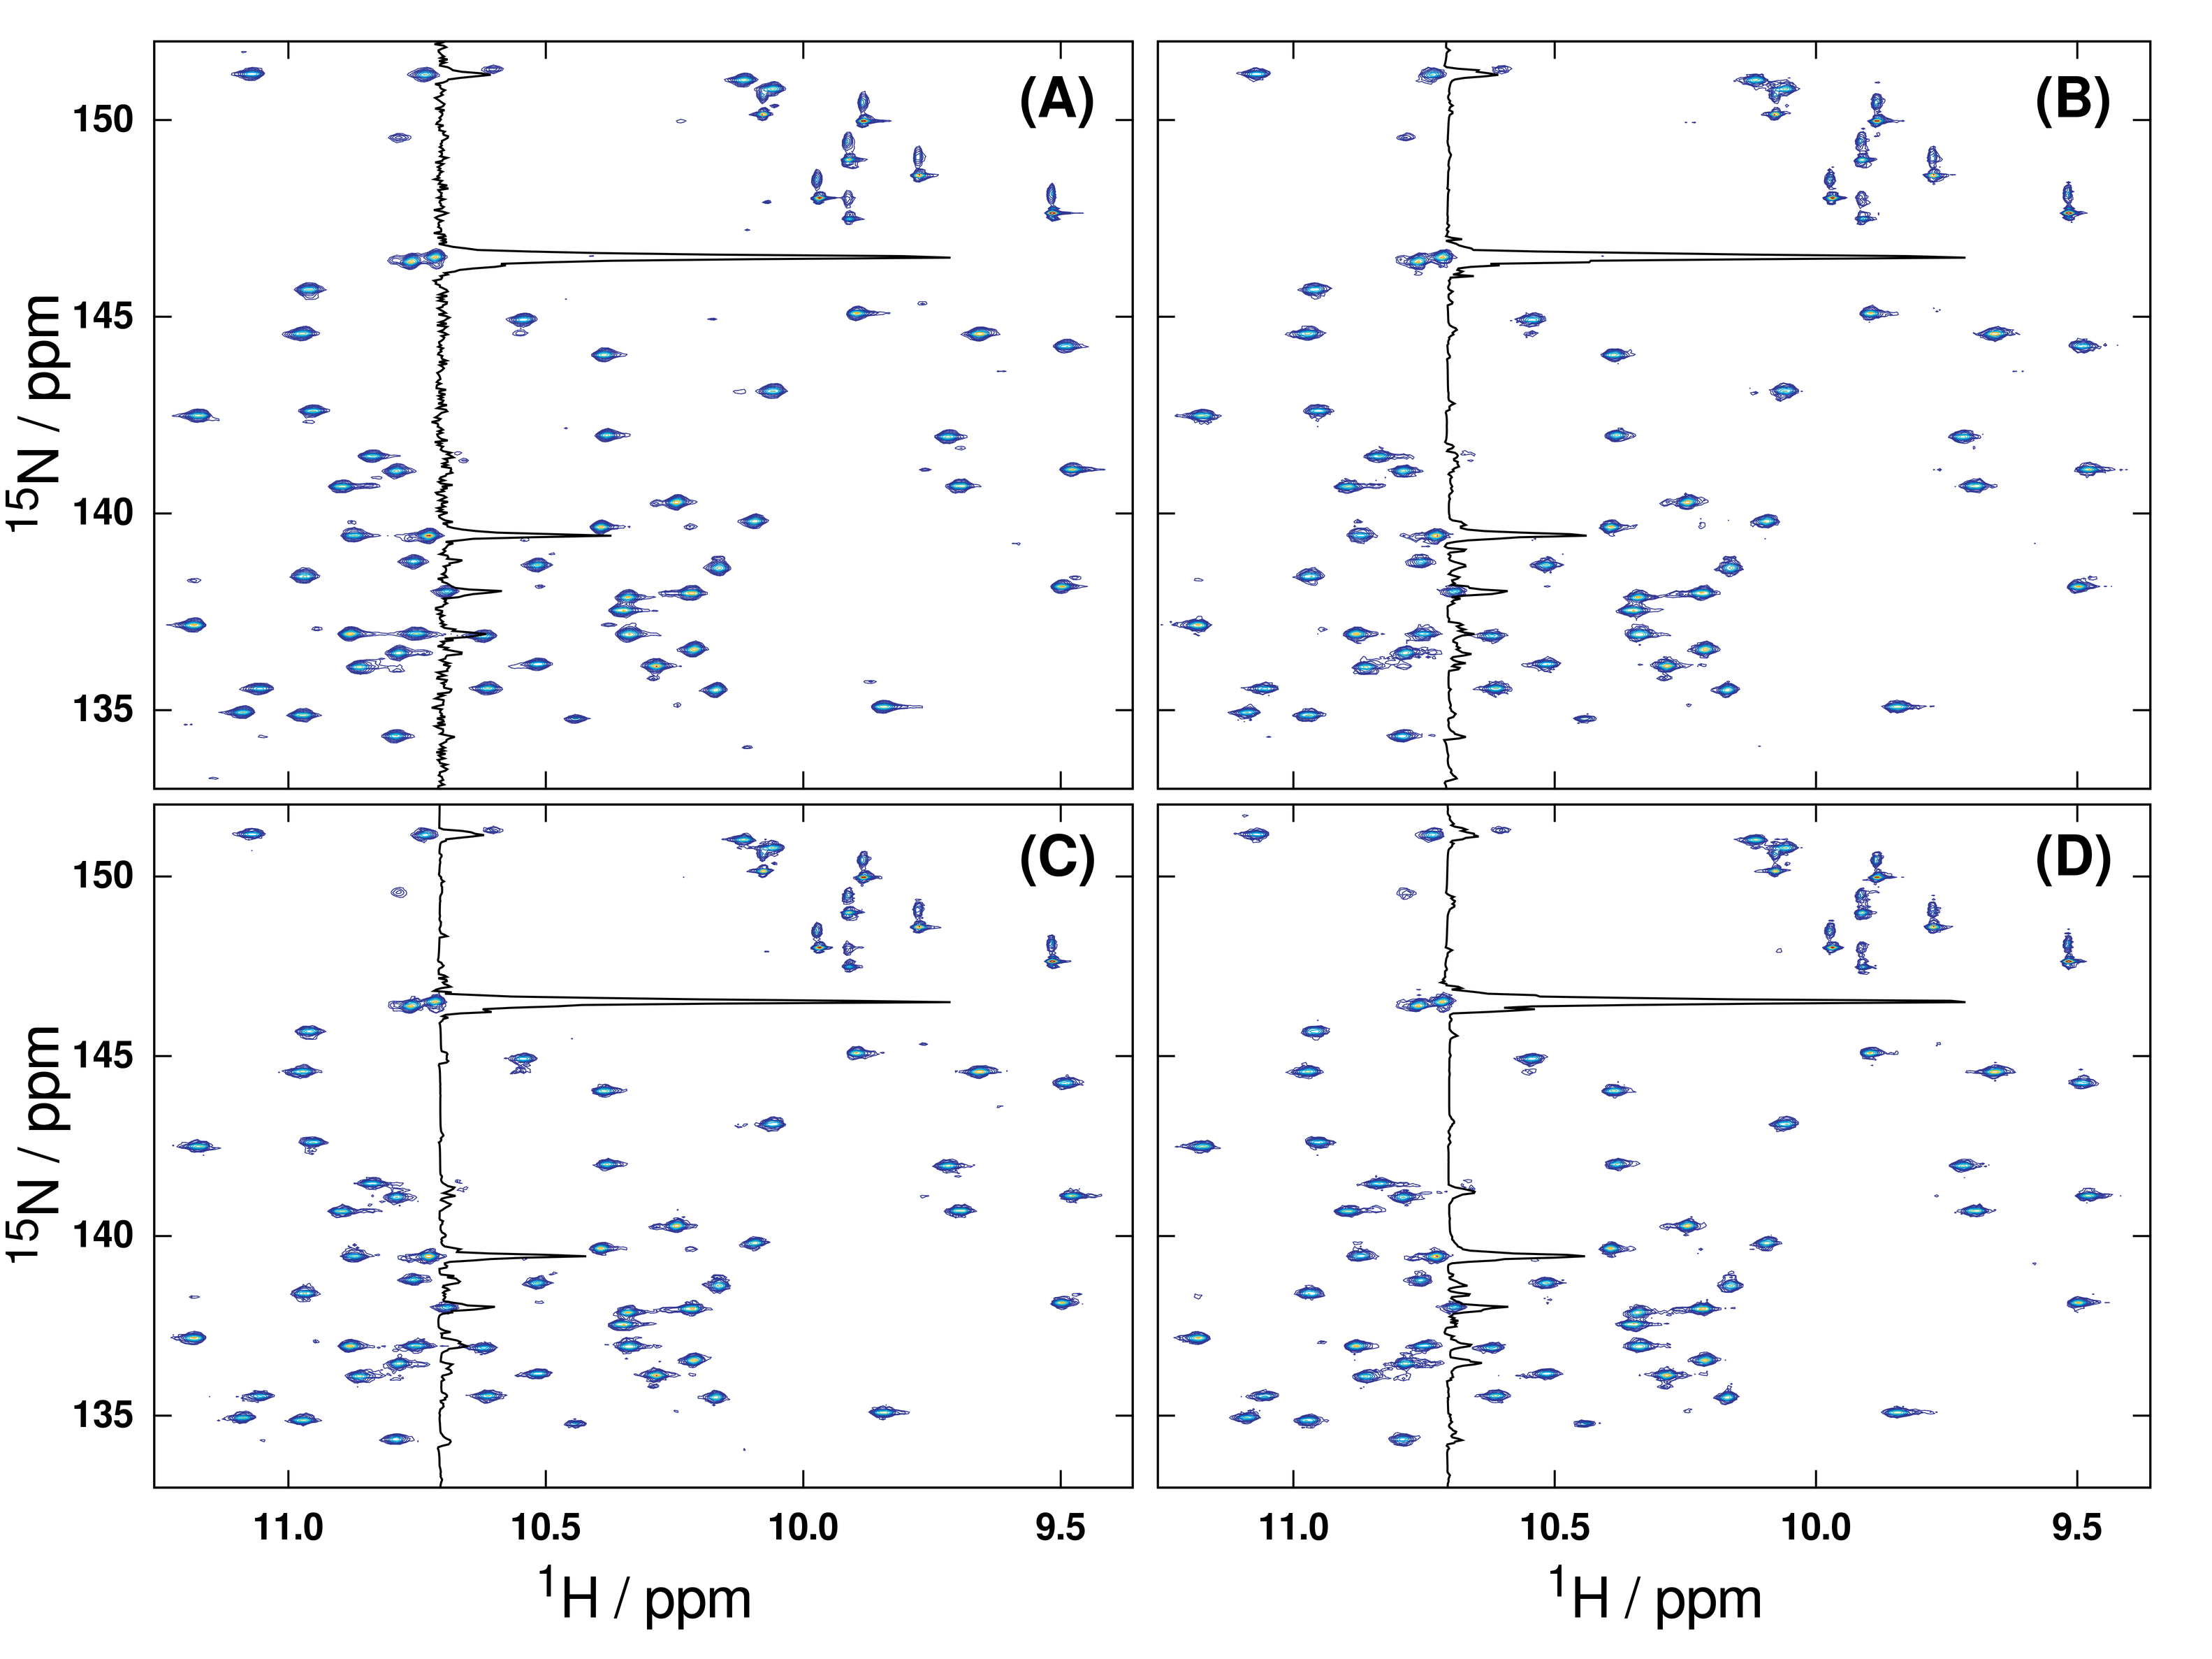
\includegraphics[width=6in]{figs/dgs/06-hsqc.png}
\caption
      [Comparison of HSQC Spectral Reconstructions.]{
  {\bf Comparison of HSQC Spectral Reconstructions.}
  \\
  Uniformly sampled ({\bf A}) and IST reconstructed ({\bf B--D}) 2D \hnnmr{}
  HSQC spectra of ubiquitin, indicating nearly equivalent performance of all
  three gap sampling methods at low (5\%) sampling density. Spectra shown in
  ({\bf B}) through ({\bf D}) were reconstructed from nonuniformly subsampled
  copies of ({\bf A}) using Poisson-gap ({\bf B}), sine-gap ({\bf C}), and
  sine-burst ({\bf D}) schedules, respectively. All spectra are plotted with
  identical contour levels.
}
\label{figure.2.6}
\end{figure}

\subsection{Spectral Data Collection}

\begin{doublespace}
A high-resolution 2D \hnnmr{} HSQC NMR spectrum was collected at a temperature
of 298.0 K on a sample of uniformly [\nnmr{}, \cnmr{}]-labeled ubiquitin in
aqueous phosphate buffer at pH 6.5. Data were acquired on a Bruker Avance
III HD 700 MHz spectrometer equipped with a 5 mm inverse quadruple-resonance
(\hnmr{}, \cnmr{}, \nnmr{}, \pnmr{}) cryoprobe with cooled \hnmr{} and \cnmr{}
channels and a $z$-axis gradient. A 2D gradient-enhanced \hnnmr{} HSQC spectrum
with improved sensitivity \cite{kay:jacs1992,palmer:jmr1991} was collected with
16 scans and 32 dummy scans over a uniform grid of 2,048 and 1,024 complex
points along the \hnmr{} and \nnmr{} dimensions, respectively. Spectral widths
were set to 3,293$\pm$4,209 Hz along \hnmr{} and 8,514$\pm$1,419 Hz along
\nnmr{}. The spectrum was windowed with a squared-cosine function,
Fourier-transformed and phase-corrected along \hnmr{} to produce a
half-transformed spectrum for IST reconstruction analysis (vide infra),
and subsequently windowed and Fourier-transformed along \nnmr{} to yield the
``true'' uniformly sampled 2D \hnnmr{} HSQC spectrum.
\figref{2.6}{Figure 2.6A} compares the true HSQC spectrum with
representative IST reconstructions after subsampling by
Poisson-gap, sine-gap and sine-burst schedules.
\end{doublespace}

\begin{figure}[ht!]
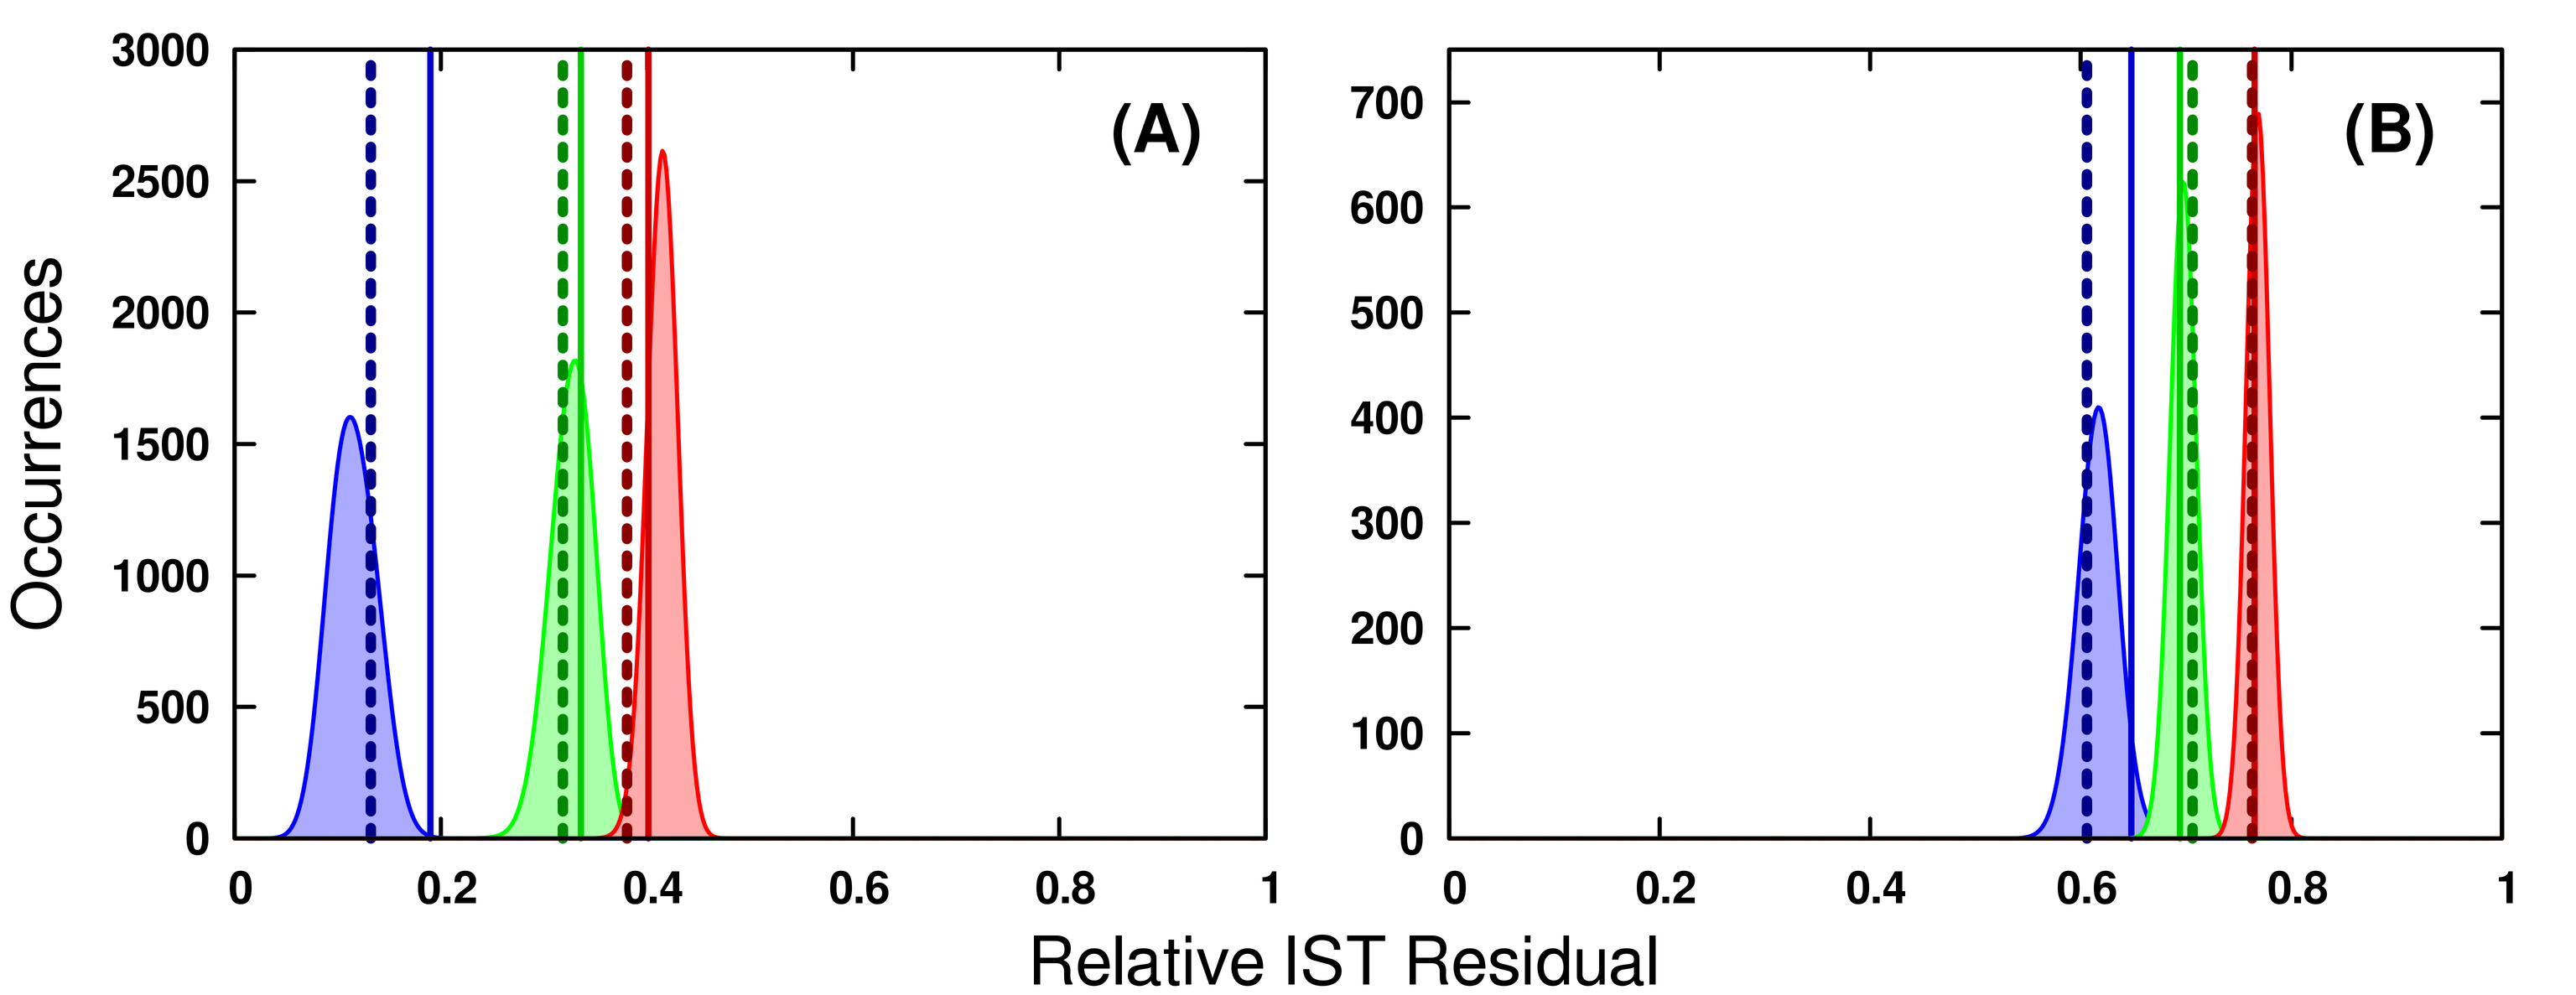
\includegraphics[width=6in]{figs/dgs/07-residuals.png}
\caption
      [Relative IST Reconstruction Residuals.]{
  {\bf Relative IST Reconstruction Residuals.}
  \\
  Iterative soft thresholding reconstruction $\ell_2$ residuals of ({\bf A})
  simulated noise-free decays and ({\bf B}) 2D \hnnmr{} HSQC slices from
  one-dimensional Poisson-gap schedules having sampling densities of
  30\% (blue), 10\% (green) and 5\% (red). Residuals of sine-gap and sine-burst
  schedules are shown as solid and dashed vertical lines, respectively.
}
\label{figure.2.7}
\end{figure}

\subsection{Computation of Performance Metrics}

\begin{doublespace}
All computational analyses were performed in GNU Octave 3.6 \cite{eaton2008}
using routines currently available in the open-source MVAPACK toolbox for
NMR chemometrics \cite{worley:acscb2014}. Impulse sets were generated for
each constructed schedule by setting sampled grid points to one and skipped
grid points to zero. At each sampling density and grid size for which schedules
were created, point-spread functions were calculated by discrete Fourier
transformation of each schedule's impulse set. Point-spread functions for
schedules built on two-dimensional grids are shown for each sampling density
in \figref{2.5}{Figure 2.5}. For one-dimensional schedules, reconstruction
residuals were computed for a noise-free synthetic free induction decay
containing a single frequency component. The synthetic decay had a normalized
frequency and decay rate of 0.04 and 0.002, respectively. The decay was
resampled according to each schedule and reconstructed with 400 iterations
of Iterative Soft Thresholding (IST) at a threshold level
of 98\% \cite{hyberts:jbnmr2012}. Following reconstruction, the residual
was calculated using the $\ell_2$-norm of the differences between the
true and reconstructed signals. \figref{2.7}{Figure 2.7A} shows the
distributions of IST reconstruction residuals for Poisson-gap, sine-gap and
sine-burst schedules. Reconstructions of the half-transformed HSQC were also
performed after nonuniformly subsampling using sine-gap schedules, sine-burst
schedules, and a subset ($N$ = 10,000) of the generated Poisson-gap schedules.
\figref{2.7}{Figure 2.7B} shows IST reconstruction residuals computed
from the HSQC spectrum.
\end{doublespace}

\begin{table}[h!]
\caption{Peak-picking Performance Figures from IST-reconstructed HSQC Spectra.}
\begin{center}
\begin{tabular}{l l | l l l l l l}
  \hline
  {\bf Method} & & {\bf Matched}       & {\bf Lost}     & {\bf Gained} &
                   $\boldsymbol{\rho}$ & $\mathbf{d_H}$ & $\mathbf{d_N}$ \\
  \hline
     & 30\% & 92/99 & 7/99 &  2 & 0.9736 & 0.003064 & 0.006165 \\
  PG & 10\% & 96/99 & 3/99 &  6 & 0.9692 & 0.003451 & 0.011702 \\
     &  5\% & 94/99 & 5/99 & 32 & 0.9751 & 0.003034 & 0.012806 \\
  \hline
     & 30\% & 93/99 & 6/99 &  3 & 0.9704 & 0.003184 & 0.005882 \\
  SG & 10\% & 96/99 & 3/99 & 13 & 0.9732 & 0.002801 & 0.011357 \\
     &  5\% & 97/99 & 2/99 & 31 & 0.9630 & 0.003450 & 0.014585 \\
  \hline
     & 30\% & 91/99 & 8/99 &  3 & 0.9820 & 0.003319 & 0.008370 \\
  SB & 10\% & 97/99 & 2/99 & 13 & 0.9820 & 0.003045 & 0.012806 \\
     &  5\% & 97/99 & 2/99 & 45 & 0.9575 & 0.003587 & 0.016998 \\
\end{tabular}
\end{center}
\end{table}

\subsection{Generation of Peak-picking Statistics}

\begin{doublespace}
For each 2D \hnnmr{} HSQC spectrum of ubiquitin reconstructed via IST at each
sampling density and each sampling method, a set of quality statistics was
computed (Table 2.1). Peak lists were generated using the
\verb peakHN.tcl  utility provided by NMRPipe \cite{delaglio:jbnmr1995}, with
a minimum intensity threshold of $3.0 \times 10^7$. Then, a greedy algorithm
was used to generate a maximum-cardinality bipartite matching between the peak
list of each reconstructed spectrum and the peak list of the true spectrum.
Chemical shift windows of 0.015 ppm and 0.08 ppm were used along the \hnmr{}
and \nnmr{} dimensions, respectively, during matching. The numbers of peaks
matched, lost and gained in the reconstructed spectra, relative to the true
spectrum, were all counted. Lost peaks were any picked peaks in the true
spectrum that had no match in the reconstruction. Gained peaks were any
picked peaks in the reconstruction with no partner in the true spectrum.
The intensities of all matched peaks in each reconstruction were then
compared against their true intensities through the computation of a Pearson
correlation coefficient, $\rho$, which effectively summarizes the linearity
of the reconstruction algorithm as a function of sampling schedule. Finally,
root-mean-square chemical shift deviations of all matched peaks along the
\hnmr{} dimension ($d_H$) and the \nnmr{} dimension ($d_N$) were also
computed.
\end{doublespace}

\begin{SCfigure}
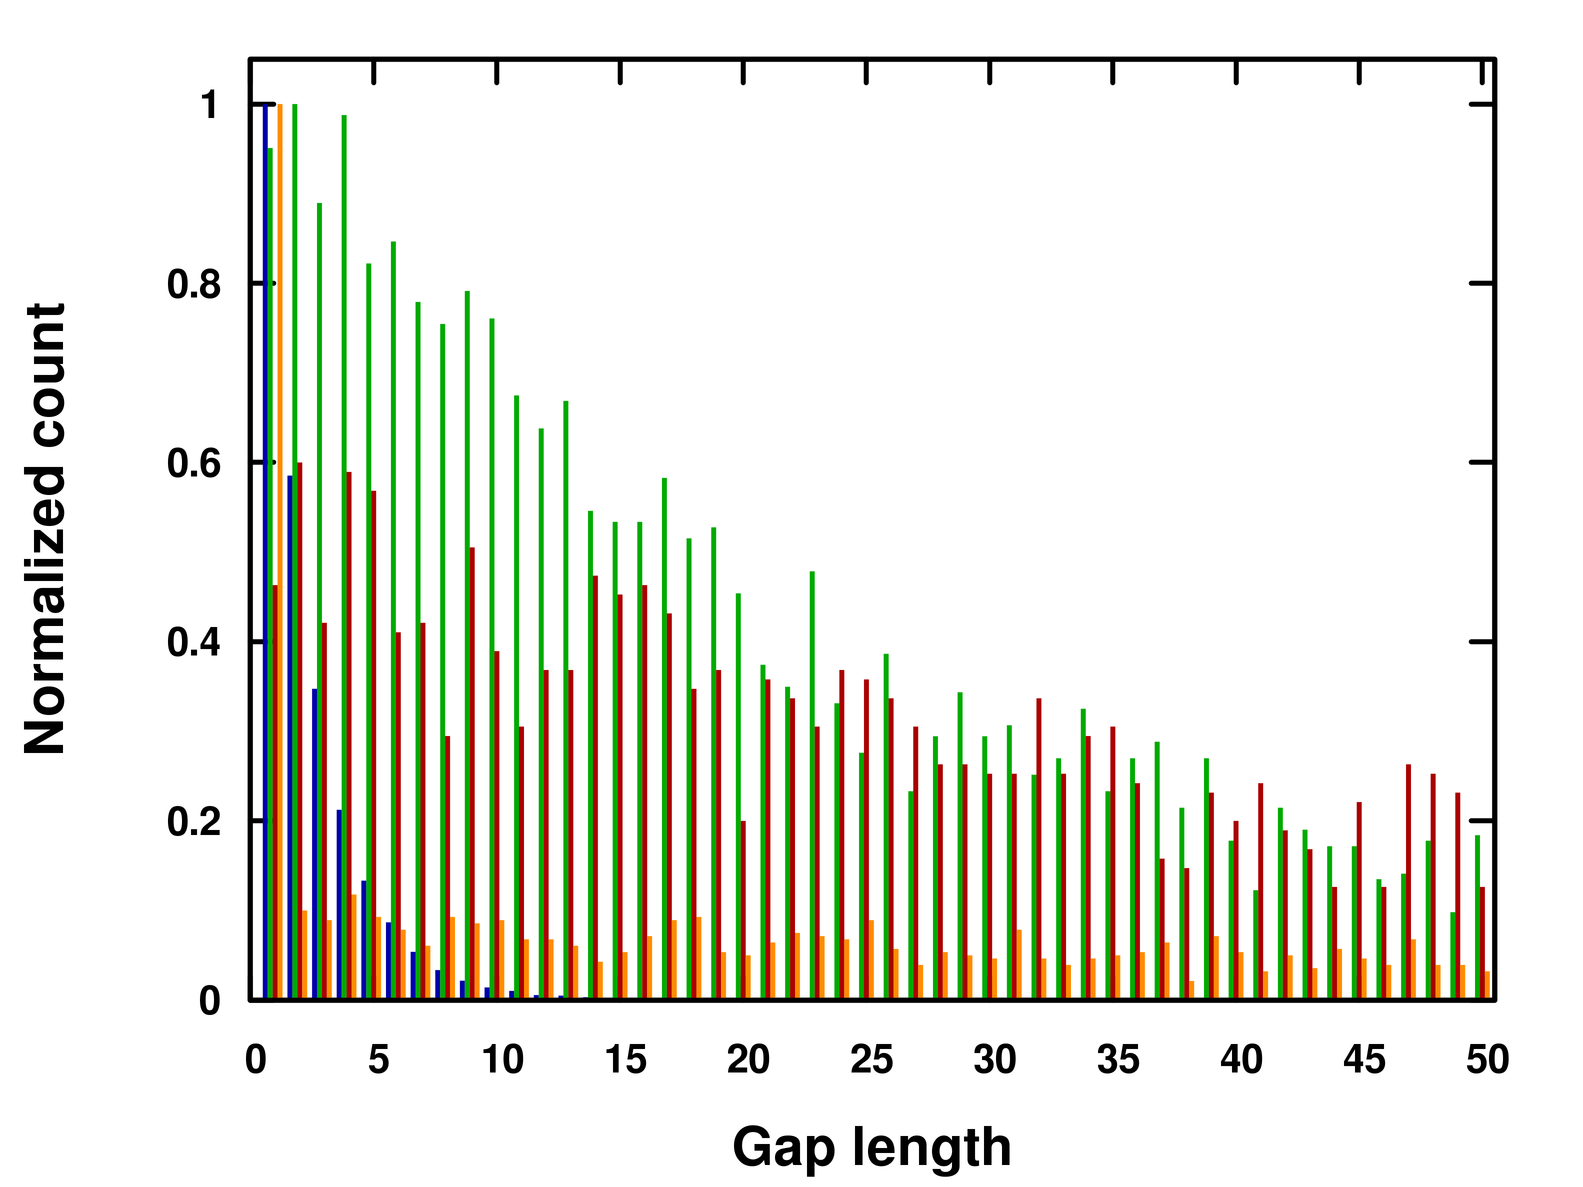
\includegraphics[width=3.25in]{figs/dgs/08-rejhist.png}
\caption
      [Gap Length Histograms from Rejection Sampling.]{
  {\bf Gap Length Histograms from Rejection Sampling.}
  \\
  Normalized histograms of gap lengths at various points in an ensemble of
  100,00 sampling schedules generated by rejection sampling from the
  Poisson-gap expectation sampling distribution (equation 2.11). Bars
  shown in blue, green, red and orange represent the gap length histograms
  at $\theta$ equal to 0.0098, 0.24, 0.73 and 0.88, respectively. Examination
  of these histograms clearly indicates that the schedules generated by
  rejection sampling are \emph{not} Poisson-gap schedules.
}
\label{figure.2.8}
\end{SCfigure}

\subsection{Analysis of Sampling Distributions}

\begin{doublespace}
Expectation sampling distributions were also generated from the set of
Poisson-gap schedules by averaging their resulting impulse sets.
\figref{2.2}{Figure 2.2} shows the expectation sampling distributions
for one-dimensional schedules having different sampling densities, and
\figref{2.3}{Figures 2.3} and \figref{2.4}{2.4} show the distributions
for two-dimensional schedules having the same densities. The heavy bias
towards early time points in Poisson-gap sampling is reaffirmed in all
figures. Sampling distributions were also computed via equations
2.11 and 2.12 for comparison to the distributions obtained by averaging
multiple impulse sets (\figref{2.2}{Figures 2.2} and \figref{2.3}{2.3}).
To verify that fully random sampling from equation 2.11 and gap sampling
from $g_{PG}$ are not equivalent, 100,000 sampling schedules were generated
by rejection sampling 51 grid points from equation 2.11 at $\Lambda=62.9$
and $N=1024$, and histograms of the gap lengths at each grid point were
computed (\figref{2.8}{Figure 2.8}). If the two methods were indeed
equivalent, one would expect the histograms in \figref{2.8}{Figure 2.8} to
resemble Poisson distributions.
\end{doublespace}

\subsection{Average Poisson-gap Sequences}

\begin{doublespace}
For \figref{2.1}{Figure 2.1}, each schedule
$\{x_1^{(m)}, x_2^{(m)},\dots, x_n^{(m)}\}$ in
the generated ensemble of $M$ (here, $M$ = 50,000)
one-dimensional Poisson-gap schedules was averaged
on a term-by-term basis:
\begin{equation}
\langle x_i \rangle = \frac{1}{M} \sum_{m=1}^M x_i^{(m)}
\end{equation}
to produce the average Poisson-gap schedule
$\{\langle x_1 \rangle, \langle x_2 \rangle,\dots, \langle x_n \rangle\}$.
Similar procedures were performed to compute the standard deviation of the
Poisson-gap ensemble. Deterministic sampling schedules with a 1x exponential
bias were computed according to procedures outlined by
Eddy et al. \cite{eddy:jmr2012}. Relative errors
(\figref{2.1}{Figure 2.1}) between a given
sine-gap schedule $\{y_1, y_2,\dots, y_n\}$ and average Poisson-gap schedule
were computed by a term-by-term subtraction of one schedule from the other,
followed by a division by the average Poisson-gap terms:
\begin{equation}
\Delta_i = \frac{y_i - \langle x_i \rangle}{\langle x_i \rangle}
 \quad \forall i \in \{1,2,\dots, n\}
\end{equation}

Relative errors between the deterministic exponential schedules and the
average Poisson-gap sequence were similarly computed.
\end{doublespace}

\begin{SCfigure}
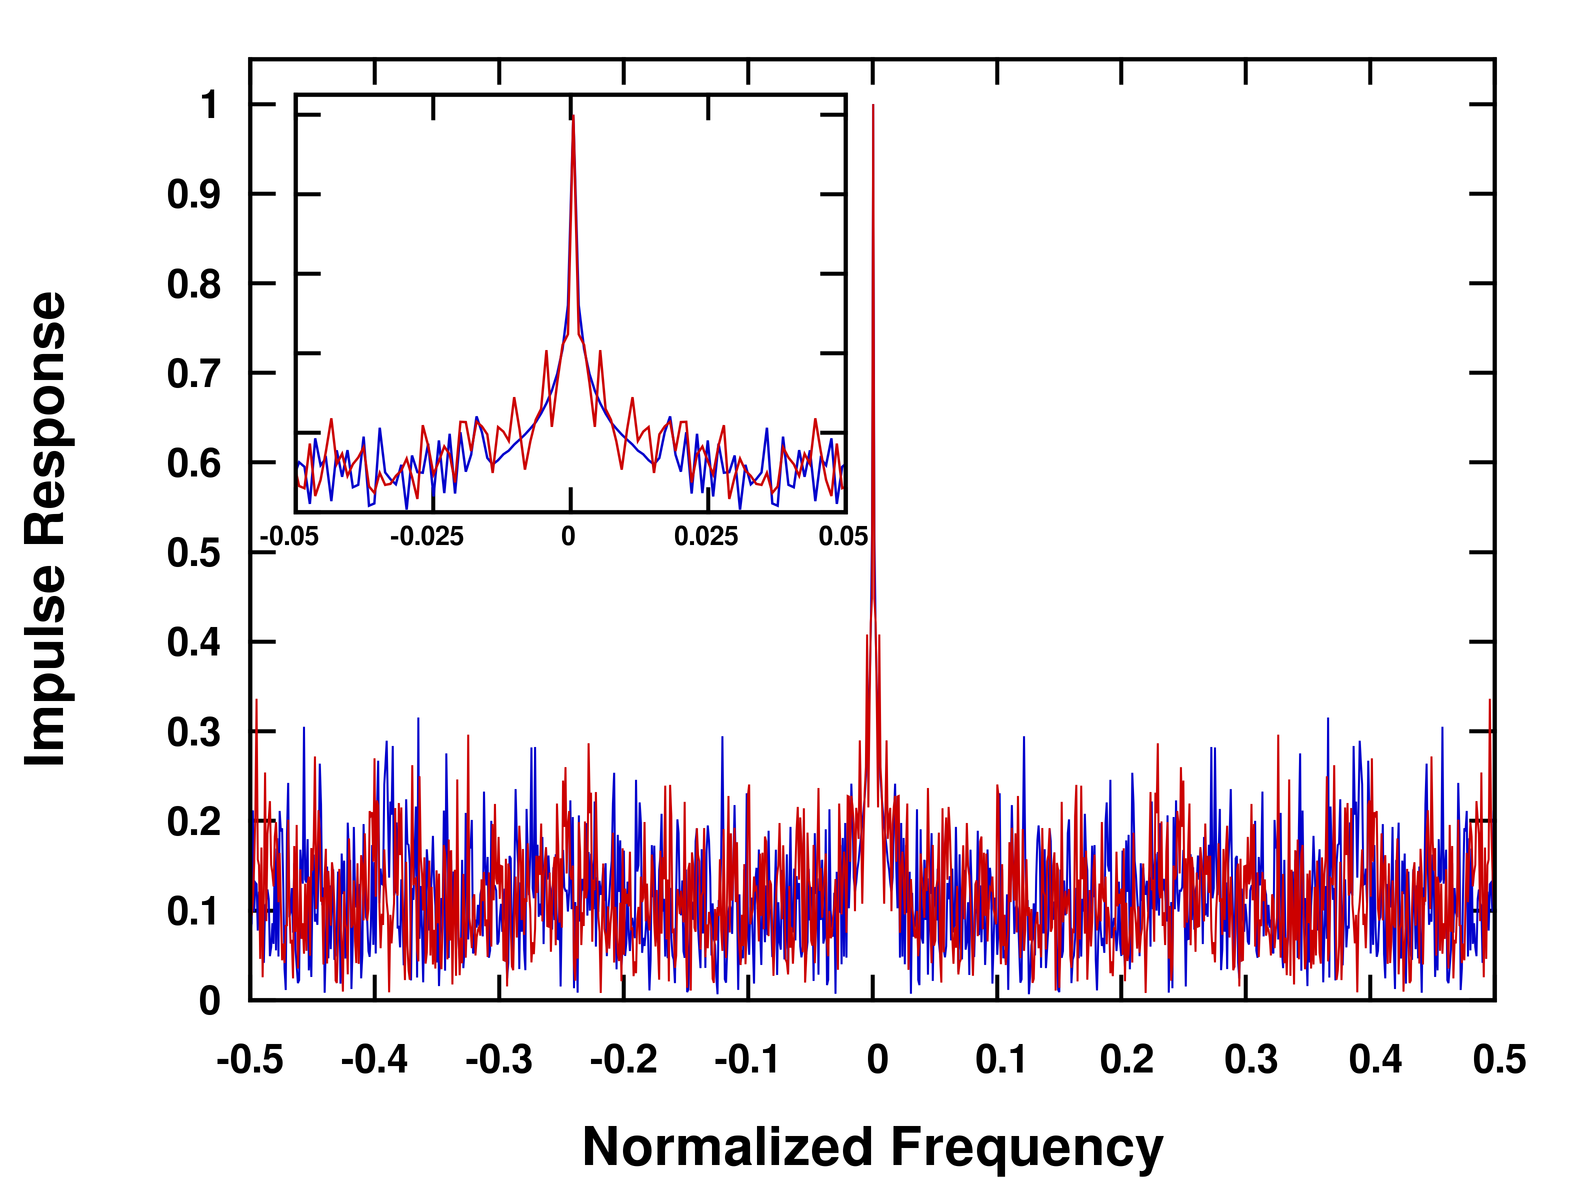
\includegraphics[width=3.25in]{figs/dgs/09-spurs.png}
\caption
      [Introduction of Spurs by Squared-sine Modulation.]{
  {\bf Introduction of Spurs by Squared-sine Modulation.}
  \\
  Impulse response functions (IRFs) of sine-gap (blue) and sine-burst (red)
  sampling schedules at 5\% density, demonstrating the appearance of
  low-frequency spurs induced by burst augmentation of the gap equation.
}
\label{figure.2.9}
\end{SCfigure}

\section{Results}

\begin{doublespace}
While at first glance, the deterministic schedule constructed using $g_{SG}$
in \figref{2.5}{Figure 2.5} may appear unrelated to the Poisson-gap
schedule, it is in fact a realization of Poisson-gap sampling in which all
random draws from the underlying Poisson distribution have resulted in the
expected value. This fact is corroborated by the corresponding point-spread
functions, which closely resemble those of the stochastic example at 30\% and
10\% sampling density. Reconstruction residuals from IST
(\figref{2.7}{Figure 2.7}) also reveal a high
similarity between the deterministic sine-gap and stochastic Poisson-gap
schedules at 30\% and 10\% density. However, the sine-gap PSF becomes less
comparable to that of Poisson-gap at low sampling densities, where the
benefits of employing random deviates are more apparent. It is worth noting
that the striking appearance of sampling artifacts in the sine-gap PSF is a
consequence of the log-scaled color gradient used in \figref{2.5}{Figure 2.5},
which was necessary in order to visually expose very low-intensity artifacts.
\\\\
The addition of burst augmentation in the form of $g_{SB}$ produces a slight
improvement in all reconstruction residuals with respect to $g_{SG}$ and
$g_{PG}$. Artifacts arising from regularity in $g_{SG}$-based schedules at
low sampling densities are diminished by burst augmentation, resulting in
point-spread functions that more closely resemble those from Poisson-gap
sampling. This reduction of artifacts by burst augmentation comes at a small
cost, at low-frequency spurs are introduced into the sine-burst point-spread
function (\figref{2.9}{Figure 2.9}) by modulating the gap equation.
However, these spurs are low in magnitude and only readily apparent at very
low (5\%) sampling density. Furthermore, IST residuals of sine-burst schedules
(\figref{2.7}{Figure 2.7}, dashed lines) are generally lower than
those of sine-gap schedules, and appear to improve relative to the mean
residuals from Poisson-gap schedules as sampling density is decreased.
Therefore, while sine-gap sampling is a valuable tool for understanding
the nature of Poisson-gap sampling, it is clearly bested in performance
by sine-burst sampling as global sampling density is decreased.
\\\\
The trade-off between minimizing the length of all gaps in a schedule, as
Poisson-gap strives to do, and minimizing the effective dwell time, as in
burst-mode sampling, is apparent by examination of gap lengths produced by
each method (\figref{2.10}{Figure 2.10}). As advertised, sine-burst
sampling schedules have decreased median gap lengths with respect to both
sine-gap and Poisson-gap schedules (\figref{2.10}{Figure 2.10A}),
at the expense of slightly increased maximum gap lengths
(\figref{2.10}{Figure 2.10B}). Rather remarkably, sine-gap schedules
have lower maximum gap lengths than their stochastic Poisson-gap cousins
\emph{and} sine-burst schedules, which reinforces the concept that the
addition of \emph{any} mechanism to reduce the greatest common factor of
the gap lengths between sampled points with force an increase in the
largest gap between points.
\end{doublespace}


\begin{figure}[ht!]
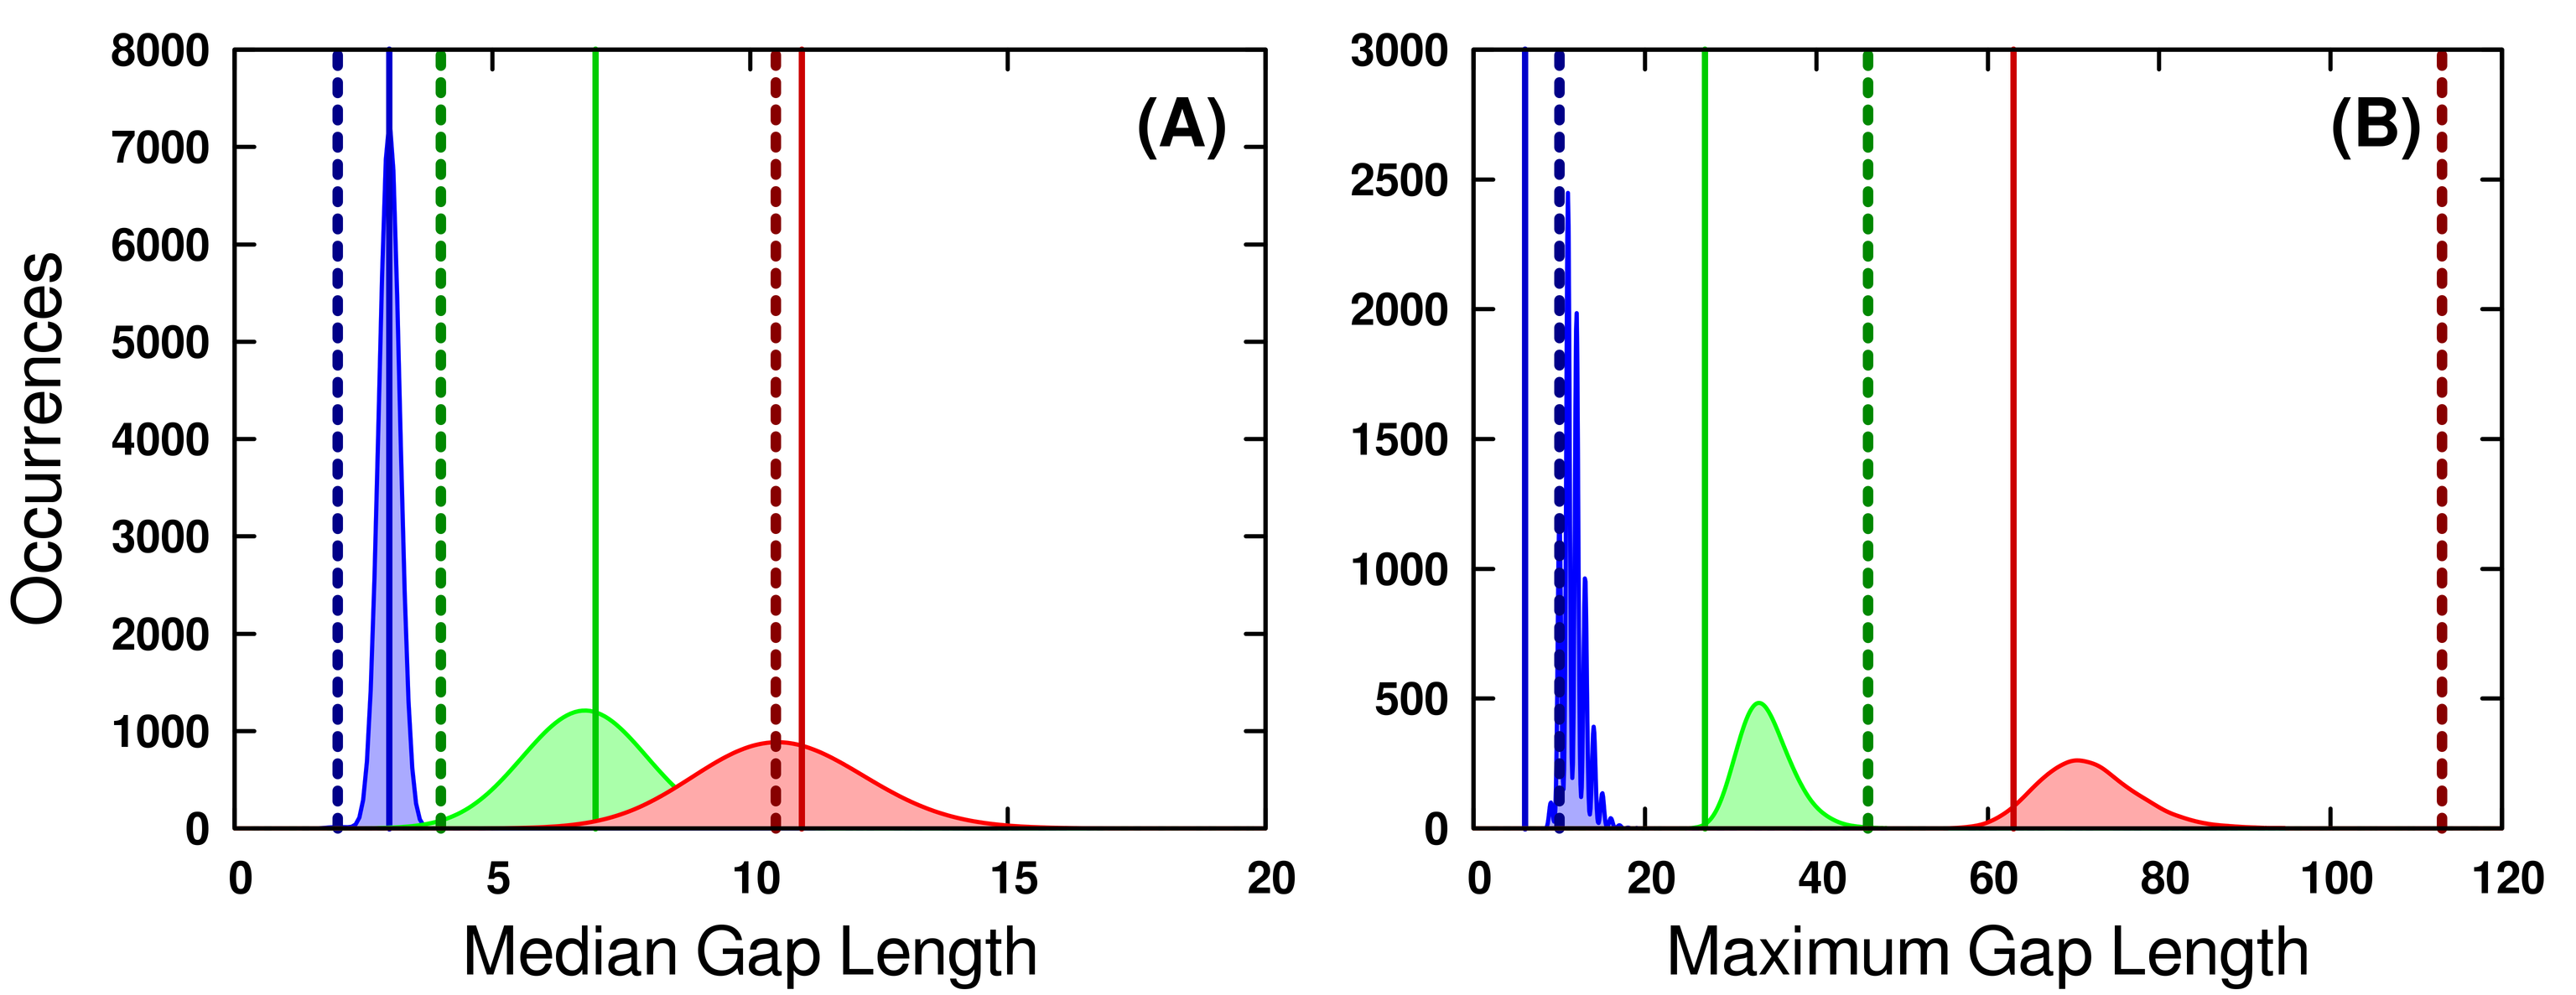
\includegraphics[width=6in]{figs/dgs/10-gaps.png}
\caption
      [Summary of Gap Lengths for all Sampling Methods.]{
  {\bf Summary of Gap Lengths for all Sampling Methods.}
  \\
  Distributions of median ({\bf A}) and maximum ({\bf B}) gap lengths from
  one-dimensional Poisson-gap schedules having sampling densities of
  30\% (blue), 10\% (green) and 5\% (red). Gap lengths of sine-gap and
  sine-burst schedules are shown as solid and dashed vertical lines,
  respectively. The gap lengths resulting from burst augmentation of the
  sine-gap equation have markedly decreased median values at the expense
  of increased maximum values, relative to sine-gap and Poisson-gap schedules.
}
\label{figure.2.10}
\end{figure}

\section{Discussion and Conclusions}

\begin{doublespace}
This chapter has shown that Poisson-gap sampling is a single instance in a
class of gap sampling methods, which may or may not be defined stochastically.
Using the well-defined gap sampling algorithm, two novel deterministic sampling
methods have been described: sine-gap and sine-burst sampling. Neither of
these new methods relies on random deviates, and both have comparable
performance to Poisson-gap sampling according to IST reconstruction residuals.
From a practical perspective, Poisson-gap, sine-gap and sine-burst sampling
methods produced nearly equivalent HSQC spectral reconstructions
(\figref{2.6}{Figure 2.6}) that yielded essentially identical
information (chemical shifts, peak
intensities) as highlighted in Table 2.1. For the practicing spectroscopist,
this equates to the ability to nonuniformly sample at the performance level
of Poisson-gap, without specifying a pseudorandom seed. Gap sampling is a
flexible and attractive alternative to traditional probabilistic sampling
methods that use probability densities to define the local sampling density
over a Nyquist grid. In effect, gap sampling approaches the problem of local
sampling density from the opposite direction of probabilistic sampling by
defining the distances \emph{between} samples on the grid. This chapter also
holds a brief derivation of the mathematical connection between stochastic
gap equations and their expectation sampling distributions, which allows for
direct visualization of the grid-point weighting produced by a given gap
equation. While these expectation sampling distributions are useful in
describing the sampling behavior of a stochastic gap equation, they do not
provide a means of converting a gap-based sampling method into a fully random
sampling method. In other words, it has been shown that any method of
constrained random sampling using a gap equation is inequivalent to fully
random sampling from its corresponding expectation sampling distribution.
\\\\
Finally, burst augmentation provides a concrete example of how deterministic
gap sampling may be tuned to behave in a similar fashion to pseudorandom
numbers. At first glance, the third row of \figref{2.5}{Figure 2.5} would
appear to have been generated stochastically, but it is a consequence of the
squared-sine modulation term in $g_{SB}$. It has historically been true that
stochastically generated sampling schedules produced fewer prominent artifacts
than deterministic methods such as radial or spiral sampling, due to high
regularity of the latter schemes. However, pseudorandom variates are
not required for effective sampling artifact suppression. Furthermore,
while most pseudorandom number generators are indeed deterministic for a
given seed value, this determinism is \emph{inherently different} from the
determinism offered by sine-gap and sine-burst sampling. By design, any
parameters (e.g. reconstruction residuals) measured from pseudorandomly
generated sampling schedules will not be smoothly varying -- and therefore
optimizable -- functions of their random seed value. As a consequence, no
absolute guarantee of spectral quality is provided to the spectroscopist
employing pseudorandom sampling schedules, even if the relative difference
in quality between the best- and worst-performing Poisson-gap seed values
is small at sampling densities above 10\%. This problem with seeds has
already been recognized: Poisson-gap and jittered sampling methods are, in
fact, two separate attempts at minimizing -- but not removing -- the effect
of seed values on schedule performance
\cite{hyberts:jacs2010,kazimierczuk:jmr2007,mobli:jmr2015}. Deterministic
gap sampling completely frees the user from specifying an arbitrary seed
value, and provides a highly general framework that enables further
investigation into which features of NUS schedules yield higher-quality
reconstruction results.
\\\\
The C implementations of Poisson-gap, sine-gap and sine-burst sampling are
free and open source software, and are available for download at
\url{http://bionmr.unl.edu/dgs.php}. The programs are highly portable and
C99 compliant, so they may be compiled on any modern operating system. An
online schedule generation tool is also provided at the same address for
rapid generation of one-, two- and three-dimensional NUS schedules suitable
for direct use on Bruker or Agilent spectrometers. As defined and implemented,
the recursive schedule generation algorithm is not limited to any number of
grid dimensions. However, the online tool has been hard-limited to 3D grids
to minimize server load.
\end{doublespace}

\bibliographystyle{abbrv}
\bibliography{bworley}

